% Para compilar, use:
% pdflatex -shell-escape softwarelivre.tex

%%%%%%%%%%%%%%%%%%%%%%%%%%%%%%%%%%%%%%%%%%%%%%%%%%%%%%%%%%%%%%%% 
% PREAMBULO
%%%%%%%%%%%%%%%%%%%%%%%%%%%%%%%%%%%%%%%%%%%%%%%%%%%%%%%%%%%%%%%%

%%%%%%%%%%
% Opções do beamer
\documentclass{beamer}
\usetheme{Boadilla}

\usefonttheme[onlysmall]{structurebold}
\setbeamerfont{frametitle}{family=\bfseries}
\setbeamerfont{title}{family=\bfseries}

\usenavigationsymbolstemplate{}

% This Charming Man palette from colorlovers.com
\definecolor{purple}{rgb}{0.5,0,0.5}
% Aqui você pode escolher as cores padrão para as estruturas do beamer
%\setbeamercolor{normal text}{fg=winterbland}
\setbeamercolor{structure}{fg=purple}
%\setbeamercolor{block title}{fg=lazereyes}
%\setbeamercolor{block body}{}
\setbeamercolor{alerted text}{fg=purple}
\setbeamercolor{frametitle}{fg=purple}

\AtBeginSection{\frame{\tableofcontents[currentsection,hideallsubsections]}}
%%%%%%%%%%


%%%%%%%%%%
% Pacotes adicionais
\usepackage[utf8]{inputenc} % Para permitir a exibição correta de acentos
\usepackage[portuguese]{babel} % Para exibir palavras-chave em português
\usepackage{txfonts} % Fontes bonitas :)
\usepackage{ctable}
%\usepackage{colortbl}
%%%%%%%%%%

% Variáveis da apresentação
\title{Software Livre\\Passado, Presente e Futuro}
\author{Melissa Weber Mendonça}
\date{SECCOM 2016}

%%%%%%%%%%%%%%%%%%%%%%%%%%%%%%%%%%%%%%%%%%%%%%%%%%%%%%%%%%%%%%%%
% FIM DO PREAMBULO
%%%%%%%%%%%%%%%%%%%%%%%%%%%%%%%%%%%%%%%%%%%%%%%%%%%%%%%%%%%%%%%%

\begin{document}

{% Definindo slide de título.
\setbeamertemplate{footline}{} 
\setbeamertemplate{headline}{}
\begin{frame}%
   \titlepage
\end{frame}%
}

% Slide 1
\begin{frame}
   \frametitle{O que é \emph{Software Livre}?}
   \begin{center}
     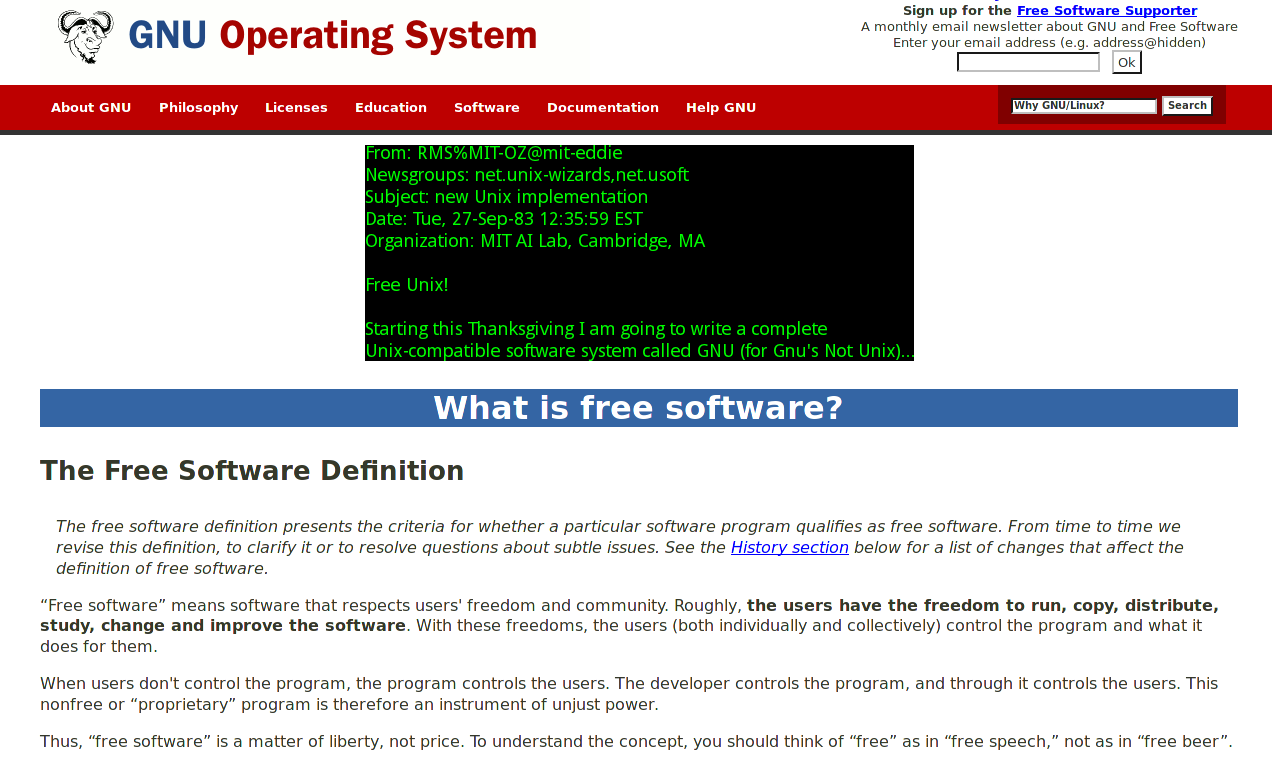
\includegraphics[width=\textwidth]{images/gnu_free.png}
   \end{center}
\end{frame}

% Slide 2
\begin{frame}
   \frametitle{Richard Stallman e o Manifesto GNU}
   \begin{columns}
     \column{6cm}
     \begin{itemize}
       \item 1983: \emph{GNU's Not Unix}
       \item 1985: Free Software Foundation
     \end{itemize}
     \column{4.5cm}
     \begin{center}
       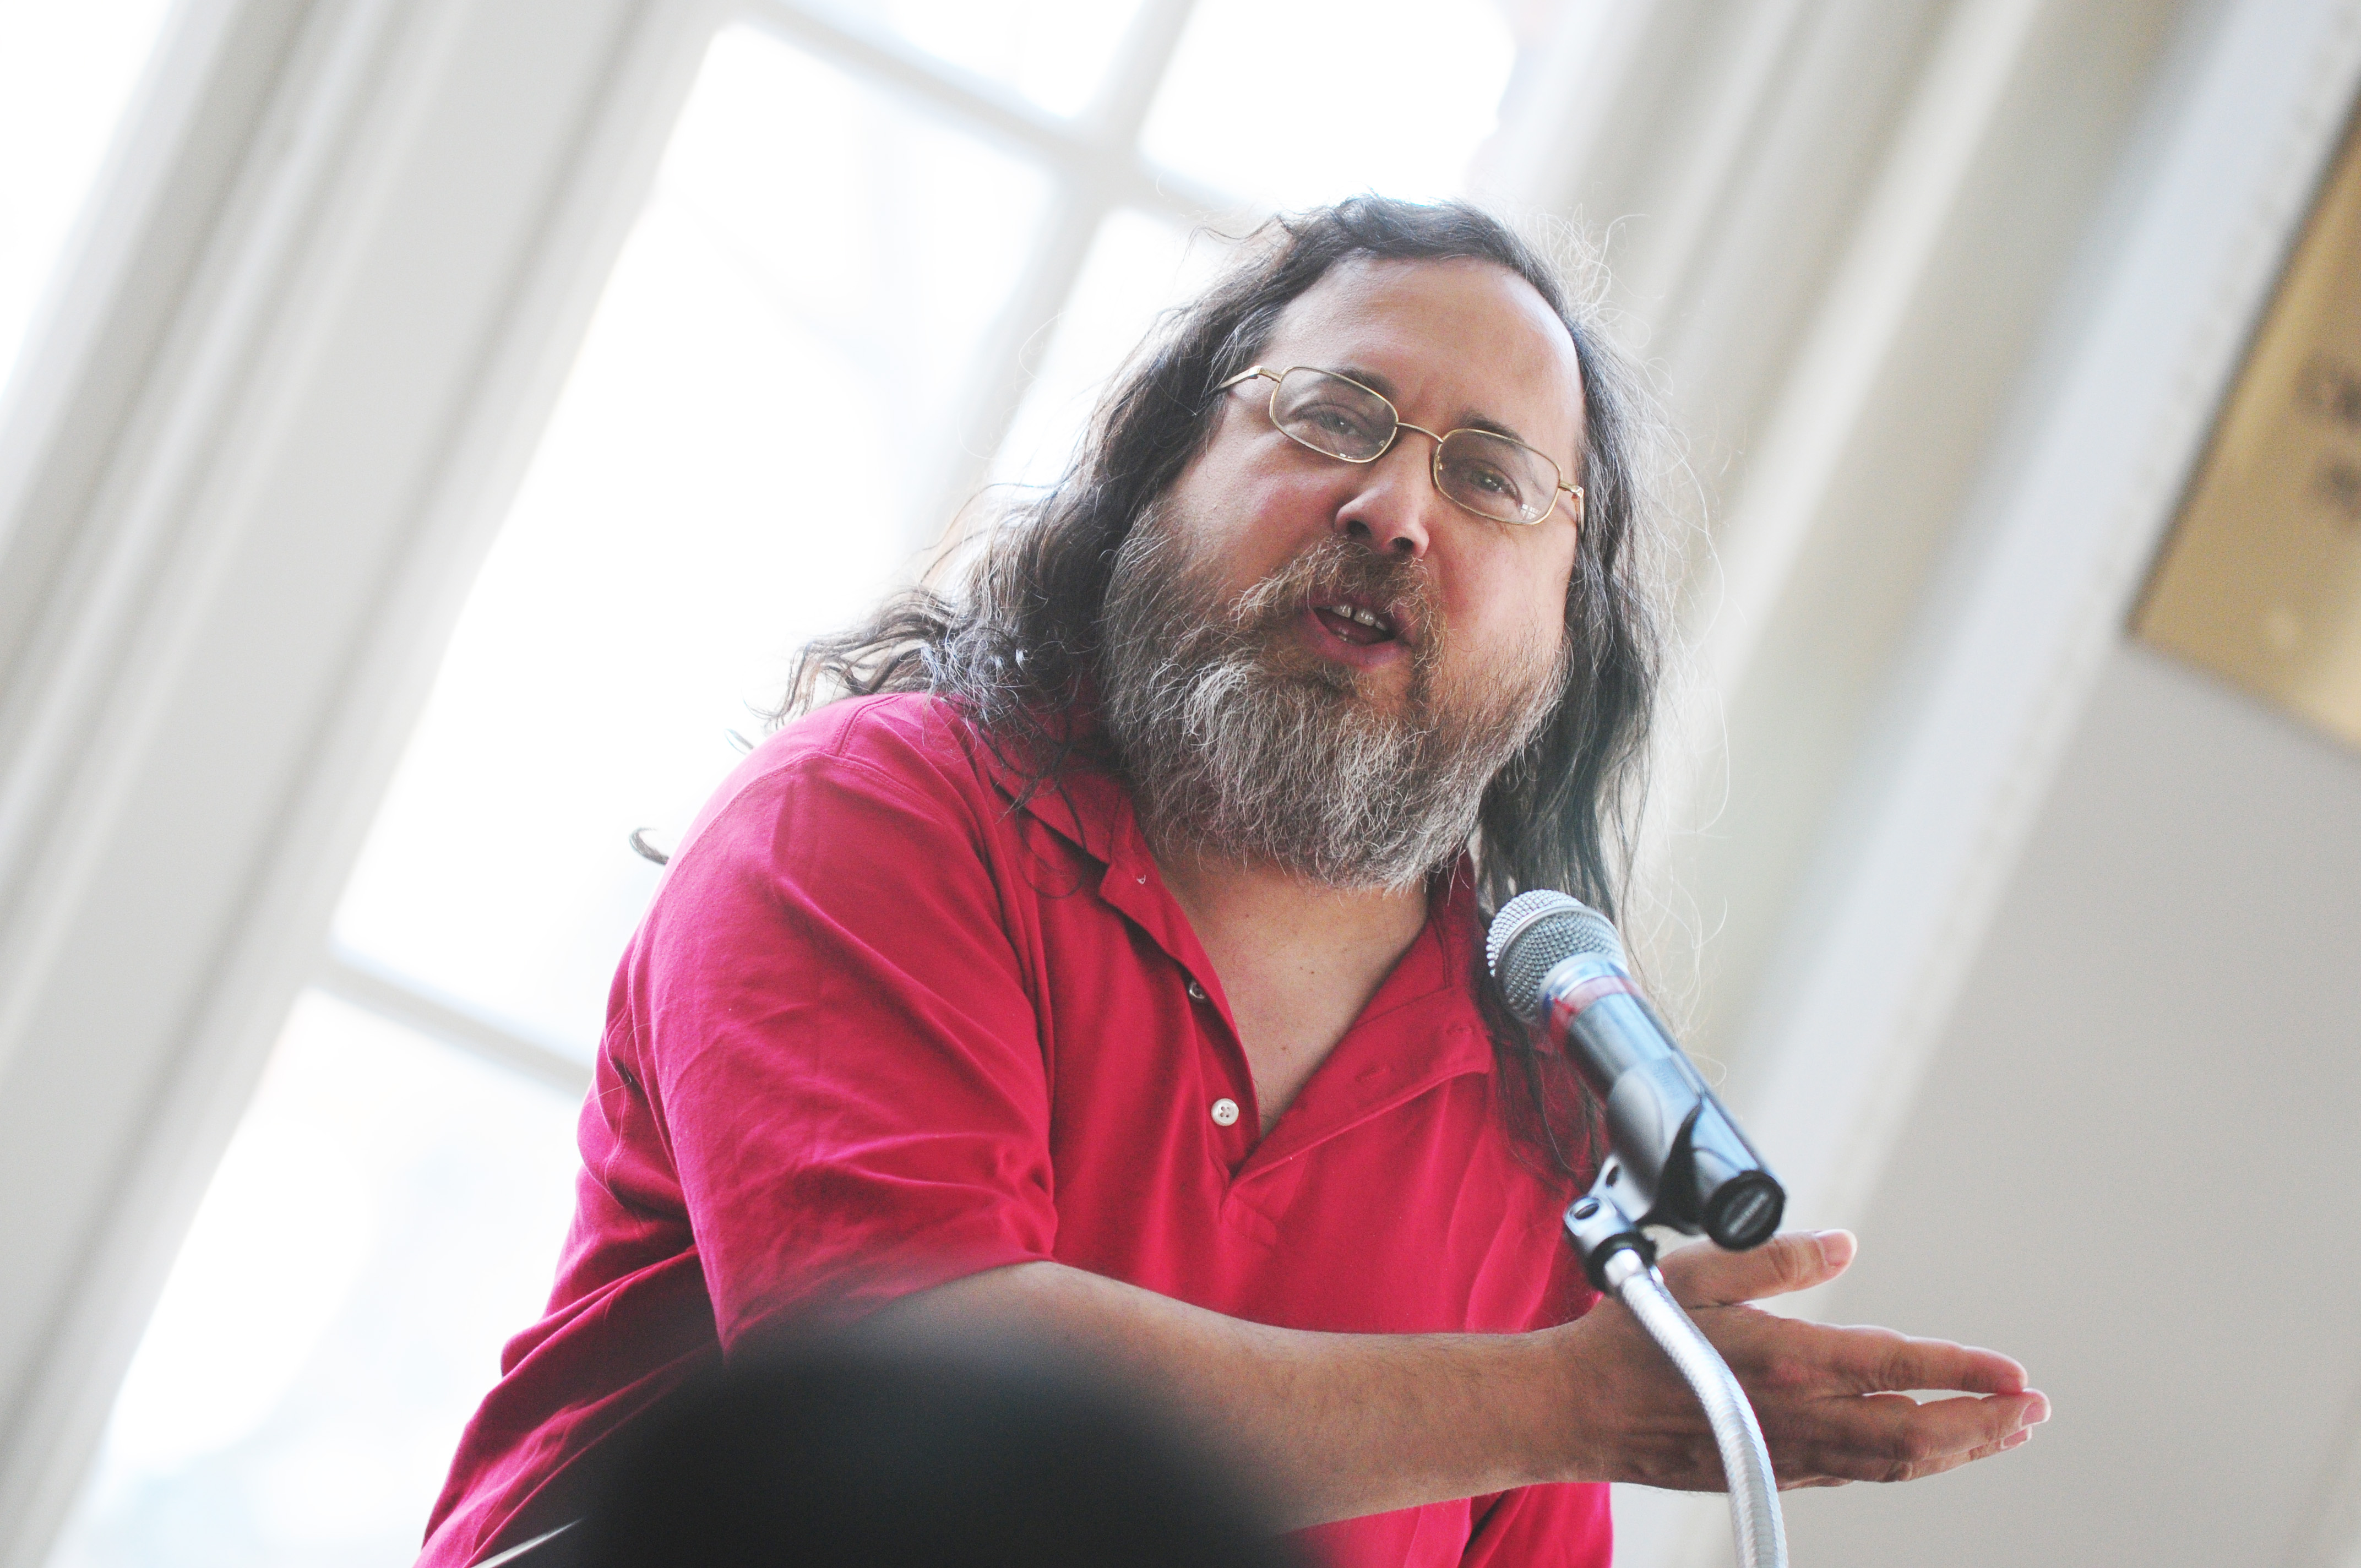
\includegraphics[width=4.5cm,trim=40mm 0mm 40mm 0mm,clip]{images/stallman.jpg}\\
       rms
     \end{center}
   \end{columns}
   \begin{center}
     ``The principal goal of GNU is to be free software. Even if GNU had no technical advantage over Unix, it would have a social advantage, allowing users to cooperate, and an ethical advantage, respecting the user's freedom.''
   \end{center}
\end{frame}

% Slide 3
\begin{frame}
  \frametitle{As liberdades}
  \begin{block}{}
  \begin{description}[<+->]
  \item[Liberdade 0] O usuário deve poder executar o programa, para qualquer fim.
  \item[Liberdade 1] O usuário deve poder estudar como o programa funciona, e fazer modificações para que o resultado seja o que ele deseja. (código aberto)
  \item[Liberdade 2] O usuário deve poder redistribuir cópias do programa para sua comunidade.
  \item[Liberdade 3] O usuário deve poder redistribuir suas cópias modificadas.
  \end{description}
  \end{block}
\end{frame}

% Slide 4
\begin{frame}
   \frametitle{\emph{``Free as in beer''} vs. \emph{``Free as in speech''}}
   \begin{center}
     \begin{minipage}{0.8\textwidth}
       \begin{block}{}
         \begin{center}
           Software Livre não é necessariamente grátis!
         \end{center}
       \end{block}
     \end{minipage}
   \end{center}
   \vfill 
   "Free software is software that gives you the user the freedom to share, study and modify it. We call this free software because \textbf{the user is free}." \textemdash\ FSF
\end{frame}

% Slide 5
\begin{frame}
   \frametitle{Licenças Livres}
   \begin{itemize}
   \item Copyleft é uma subversão da lei de copyright: ao invés de restringir um programa, exige que ele seja livre.
   \item Impede que alguém faça uma modificação a um software livre e aplique uma licença proprietária.
   \item Contagiosa: impede que se combine software livre e proprietário com uma licença proprietária
   \end{itemize}
   \begin{columns}
     \column{4cm}
     \begin{center}
       
\includegraphics[width=3cm]{images/copyleft.png}
     \end{center}
     \column{7cm}
     \begin{center}
       
\includegraphics[width=5cm]{images/GPLv3_Logo.png}
     \end{center}
 \end{columns}
\end{frame}

% Slide 6
\begin{frame}
  \frametitle{Licenças Livres}
  \begin{itemize}
  \item Apache
  \item BSD
  \item LaTeX Project Public License
  \item Microsoft Public License (Ms-PL)
  \item Mozilla Public License (MPL)
  \item Domínio Público
  \item Creative Commons
  \end{itemize}
\end{frame}

% Slide 7 - não usado na SECCOM
% \begin{frame}
%   \frametitle{Creative Commons}
%   Para trabalho artístico ou criativo (fotos, imagens, música, produção literária...)
%   \begin{itemize}
%   \item CC BY: Atribuição; trabalho pode ser modificado e a modificação pode ser usada comercialmente;
%   \item CC BY-SA: CC BY + deve manter a mesma licença do original (copyleft);
%   \item CC BY-ND: Atribuição; trabalho pode ser comercializado e redistribuído, mas sem modificações;
%   \item CC BY-NC: Atribuição; trabalho pode ser modificado e redistribuído, não comercialmente.
%   \item CC BY-NC-SA
%   \item CC BY-NC-ND
%   \end{itemize}
% \end{frame}

% Slide 8
\begin{frame}
   \frametitle{Open Source vs. Free Software}
   \begin{columns}
     \column{8cm}
     \begin{center}
     Todo software livre é \emph{open source} (código aberto) mas nem todo código aberto é software livre!\\
     \vskip2cm
     
\includegraphics[width=2cm]{images/osi-logo.png}
   \end{center}
   \column{3cm}
   \begin{center}
     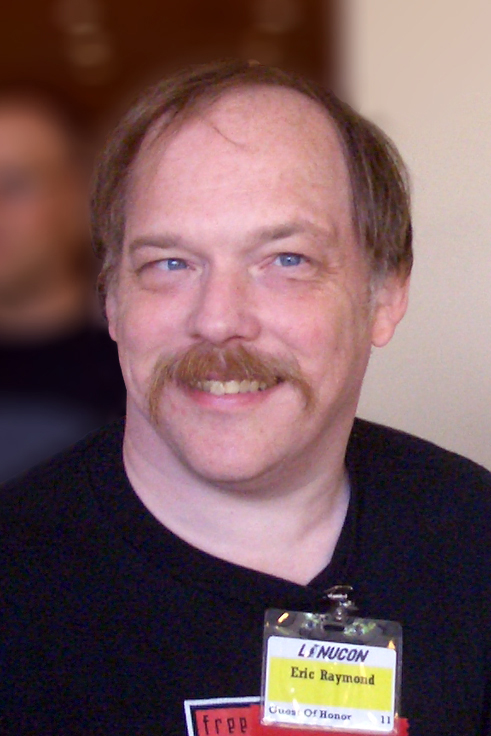
\includegraphics[width=3cm]{images/esr.jpg}\\
     Eric S. Raymond (1998)
   \end{center}
 \end{columns}
\end{frame}

% Slide 9
\begin{frame}
  \frametitle{GNU/Linux}
  \begin{center}
    \begin{minipage}{0.8\textwidth}
      \begin{block}{}
        \begin{center}
          “Every good work of software starts by scratching a developer's personal itch.” - esr
        \end{center}
      \end{block}
    \end{minipage}
  \end{center}
  \begin{columns}
    \column{7cm}
      ``Hello everybody out there using minix — I’m doing a (free) operating
      system (just a hobby, won’t be big and professional like gnu)...''
    \column{3cm}
    \begin{center}
      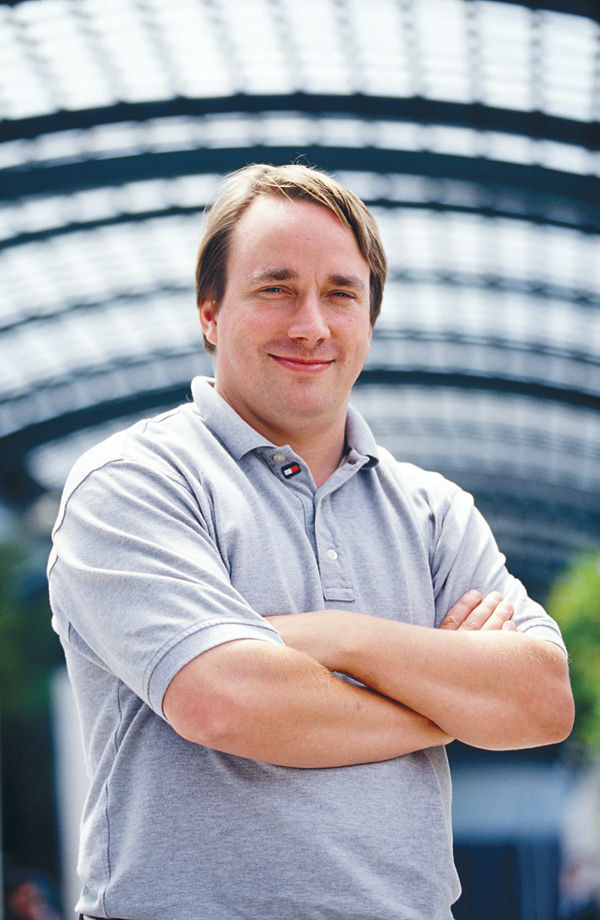
\includegraphics[width=3cm]{images/linus.jpg}\\
      Linus Torvalds\\
      (1991-1992)
    \end{center}
  \end{columns}
\end{frame}

% Slide 10 - acrescentei manjaro
\begin{frame}
   \frametitle{\emph{Distros}}
   \begin{center}
     \renewcommand\arraystretch{2}
     \begin{tabular}{c c c}
       
\includegraphics[width=3cm]{images/ubuntu.png} & 
\includegraphics[width=3cm]{images/opensuse.png} & 
\includegraphics[width=3cm]{images/mint.jpg}\\
       
\includegraphics[width=3cm,trim=10mm 60mm 10mm 60mm,clip]{images/fedora.jpg} & 
\includegraphics[width=3cm]{images/debian.png} & 
\includegraphics[width=3cm]{images/arch.png}\\
       
\includegraphics[width=3cm]{images/slack.png} & 
\includegraphics[width=3cm]{images/redhat.jpg} & 
\includegraphics[width=3cm]{images/chakra.png}\\
       
\includegraphics[width=2cm]{images/Scientific_Linux_logo.png} & 
\includegraphics[width=3cm]{images/manjaro.png} & 
     \end{tabular}
   \end{center}
\end{frame}

% Slide 11 - não usado na SECCOM
% \begin{frame}
%   \frametitle{}
%   \begin{center}
%     Ok, mas... E nós?
%   \end{center}
% \end{frame}

% Slide 12
\begin{frame}
  \frametitle{Formatos Abertos}
  \begin{columns}
    \column{7cm}
    \begin{itemize}
    \item Disseminação do conhecimento
    \item Garantia para o futuro
    \end{itemize}
    \column{4cm}
    \begin{center}
      
\includegraphics[width=3cm]{images/opendocumentformat.png}
    \end{center}
  \end{columns}
\end{frame}

% Slide 13
\begin{frame}
  \frametitle{Cultura Hacker na Educação}
  \begin{columns}
    \column{8cm}
    \begin{itemize}
    \item Ética Hacker
    \item Nelson Pretto (UFBA): ``Por uma cultura hacker na educação''
    \end{itemize}
    \column{3cm}
    
\includegraphics[width=3cm]{images/glider.png}
  \end{columns}
\end{frame}

% Slide 14
\begin{frame}
   \frametitle{Open Science}
   \begin{center}
     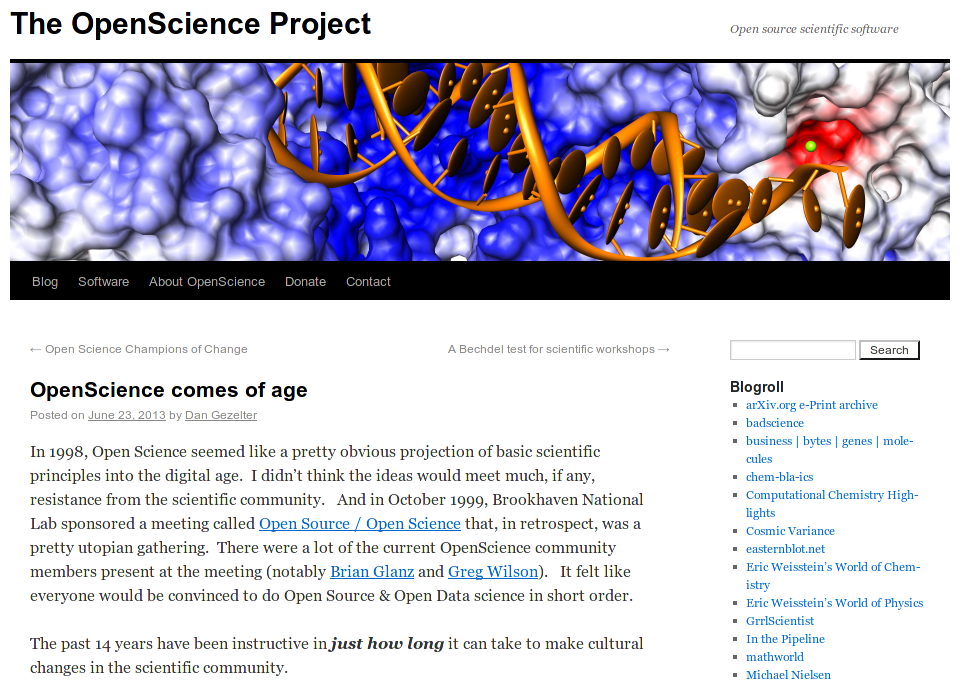
\includegraphics[width=\textwidth]{images/openscience.png}
   \end{center}
\end{frame}

% Slide 15
\begin{frame}
   \frametitle{Open Access/Open Knowledge/Open Data}
   \begin{columns}
     \column{4cm}
     \begin{center}
       
\includegraphics[width=2cm]{images/openaccess.png}\\
	\end{center}
    \column{5cm}
    \begin{center}
	
\includegraphics[width=4.5cm]{images/Open_Knowledge_logo.png}
     \end{center}
   \end{columns}
\end{frame}

% Slide 16 - novo (SECCOM)
\begin{frame}
  \frametitle{E o que a pirataria tem a ver com isso?}
  \begin{itemize}
  \item Copyright v. Copyleft
  \end{itemize}
  \vfill
  \begin{center}
    \begin{columns}
      \column{2cm}
      {\ }
      \column{5cm}
      \includegraphics[width=3cm]{images/Piratpartiet.png}
      \column{6cm}
      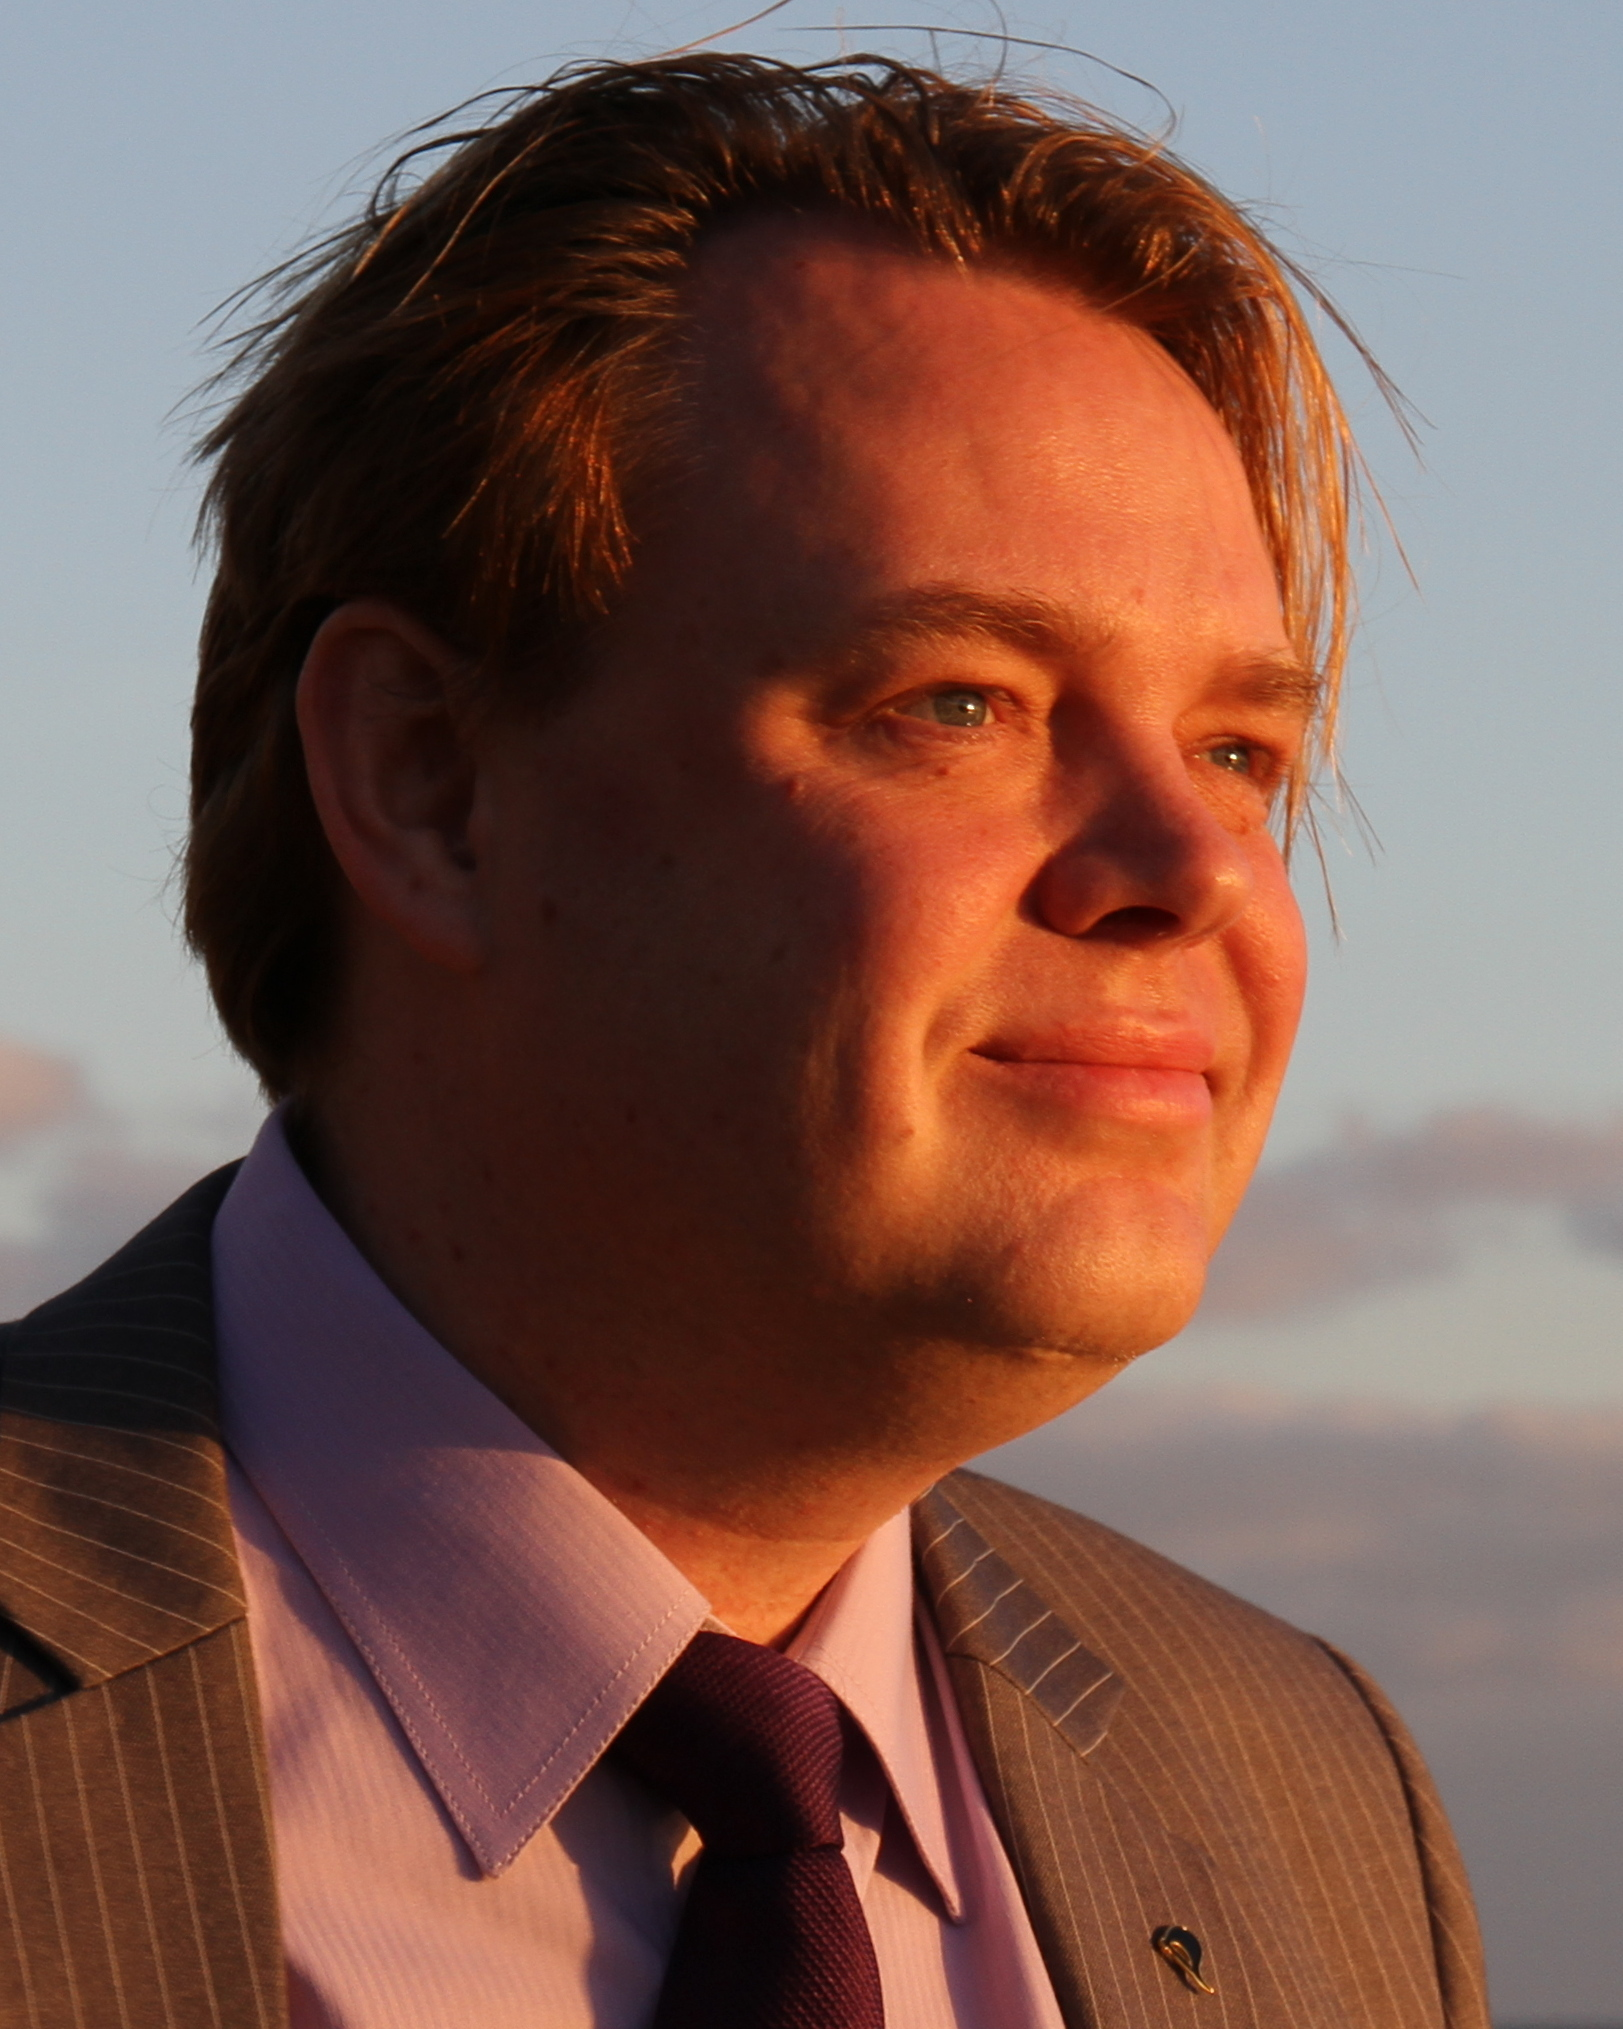
\includegraphics[width=3cm]{images/Rick_Falkvinge.jpg}
    \end{columns}
  \end{center}
\end{frame}

% Slide 17 - novo (SECCOM)
\begin{frame}
  \frametitle{Digital rights}
  \begin{columns}
    \column{4cm}
    \begin{itemize}
    \item Open Data
    \item IoT
    \end{itemize}
    \column{4cm}
    
\includegraphics[width=4cm]{images/EFF_Logo.png}
  \end{columns}
\end{frame}

% Slide 18 - não usado na SECCOM
% \begin{frame}
%    \frametitle{Softwares Matemáticos Livres}
%    \begin{center}
%      \begin{tabular}{l l}
%        \rowcolor{purple!30} MATLAB & \uncover<2->{Octave/Scilab/Python}\\
%        Photoshop & \uncover<3->{Inkscape/Gimp}\\
%        \rowcolor{purple!30} Word/Excel & \uncover<4->{LibreOffice (\LaTeX !)}\\
%        Geogebra & \uncover<5->{Geogebra :)}\\
%        \rowcolor{purple!30} Maple & \uncover<6>{Sage}
%      \end{tabular}
%    \end{center}
% \end{frame}

% Slide 19
\begin{frame}
   \frametitle{Comunidade}
   Todos podem contribuir!
   \begin{itemize}
   \item Código
   \item Tradução
   \item Acessibilidade
   \item Bugs
   \item Evangelismo
   \end{itemize}
\end{frame}

% Slide 20
\begin{frame}[fragile]
  \frametitle{Contato}
  \begin{center}
    \begin{minipage}{0.7\textwidth}
      \begin{block}{}
        \begin{center}
          % \verb+@melissawm+\\
          \verb+www.mtm.ufsc.br/~melissa+
          \verb+melissa.mendonca@ufsc.br+
        \end{center}
      \end{block}
    \end{minipage}
  \end{center}
\end{frame}

\end{document}
